\documentclass[xcolor=pdftex,dvipsnames,table,mathserif]{beamer}
\usetheme{focus}
%\usetheme{Darmstadt}
%\usepackage{times}
%\usefonttheme{structurebold}

\usepackage[english]{babel}
%\usepackage[table]{xcolor}
\usepackage{pgf,pgfarrows,pgfnodes,pgfautomata,pgfheaps}
\usepackage{amsmath,amssymb,setspace,centernot}
\usepackage[latin1]{inputenc}
%\usepackage[T1]{fontenc}
\usepackage{relsize}
\usepackage{pdfpages}
\usepackage[absolute,overlay]{textpos} 


\newenvironment{reference}[2]{% 
  \begin{textblock*}{\textwidth}(#1,#2) 
      \footnotesize\it\bgroup\color{red!50!black}}{\egroup\end{textblock*}} 

\DeclareMathSizes{10}{10}{6}{6} 
\AtBeginSection[]{
  \begin{frame}
  \vfill
  \centering
  \begin{beamercolorbox}[sep=8pt,center,shadow=true,rounded=true]{title}
    \usebeamerfont{title}\insertsectionhead\par%
  \end{beamercolorbox}
  \vfill
  \end{frame}
}
\begin{document}
\title{Multinomial Discrete Choice}
\author{Chris Conlon}
\institute{Applied Econometrics II}
\date{\today}

\frame{\titlepage}


\begin{frame}
\frametitle{Motivation}
Most decisions agents make are not necessarily binary:
\begin{itemize}
\item Choosing a level of schooling (or a major).
\item Choosing an occupation.
\item Choosing a partner.
\item Choosing where to live.
\item Choosing a brand of (yogurt, laundry detergent, orange juice, cars, etc.).
 \end{itemize}
\end{frame}

\begin{frame}
\frametitle{Nonparametric Setup}
We consider a \alert{multinomial discrete choice}:
\begin{itemize}
\item in period $t$
\item with $J_t$ alternatives.
\item subscript individual agents by $i$.
\item agents choose $j \in J_t$ with probability $P_{ijt}$.
\item Agent $i$ receives utility $U_{ij}$ for choosing $j$.
\item Choice is exhaustive and mutually exclusive.
 \end{itemize}\pause
Consider the simple example $(t=1)$:
\begin{eqnarray*}
P_{ij} = Prob( U_{ij} > U_{ik} \quad \forall j \neq k)
\end{eqnarray*}
\end{frame}

\begin{frame}
\frametitle{Nonparametric Setup}
Now consider separating the utility into the observed $V_{ij}$ and unobserved components $\varepsilon_{ij}$.
\begin{eqnarray*}
P_{ij} &=& Prob( U_{ij} > U_{ik} \quad \forall j \neq k)\\
 &=& Prob( V_{ij} + \varepsilon_{ij} > V_{ik} + \varepsilon_{ik} \quad \forall j \neq k)\\
 &=& Prob( \varepsilon_{ij}-\varepsilon_{ik} > V_{ik} - V_{ij} \quad \forall j \neq k)
\end{eqnarray*}
\pause
It is helpful to define $f(\varepsilon_{i})$ as the $J$ vector of individual $i$'s unobserved utility.
\begin{eqnarray*}
P_{ij} &=& Prob( \varepsilon_{ij}-\varepsilon_{ik} > V_{ik} - V_{ij} \quad \forall j \neq k)\\
&=& \int I( \varepsilon_{ij}-\varepsilon_{ik} > V_{ik} - V_{ij} ) f( \varepsilon_i) \partial \varepsilon_i \\
\end{eqnarray*}
\end{frame}

\begin{frame}
\frametitle{Nonparametric Setup}
In order to compute the choice probabilities, we must perform a $J$ dimensional integral over $f(\varepsilon_i)$.
\begin{eqnarray*}
P_{ij} &=&  \int I( \varepsilon_{ij}-\varepsilon_{ik} > V_{ik} - V_{ij} ) f( \varepsilon_i) \partial \varepsilon_i 
\end{eqnarray*}
There are some choices that make our life easier
\begin{itemize}
\item Multivariate normal: $\varepsilon_i  \sim N(0,\Omega)$. $\longrightarrow$ \alert{ multinomial probit}.
\item Gumbel/Type 1 EV: $f(\varepsilon_i) = e^{-\varepsilon_{ij}}  e^{-e^{-\varepsilon_{ij}}}  $ and $F(\varepsilon_i) = 1- e^{-e^{-\varepsilon_{ij}}}$ $\longrightarrow$ \alert{multinomial logit}
\item There are also heteroskedastic variants of the Type I EV/ Logit framework.
\end{itemize}
\end{frame}

\begin{frame}
\frametitle{Errors}
Allowing for full support $[-\infty, \infty]$ errors provide two key features:
\begin{itemize}
\item Smoothness: $P_{ij}$ is everywhere continuously differentiable in $V_{ij}$.
\item Bound $P_{ij} \in (0,1)$ so that we can rationalize any observed pattern in the data.
\item What does $\varepsilon_{ij}$ really mean? (unobserved utility, idiosyncratic tastes, etc.)
\end{itemize}
\end{frame}

\begin{frame}
\frametitle{Basic Identification}
\small
\begin{itemize}
\item Only differences in utility matter: $Prob( \varepsilon_{ij}-\varepsilon_{ik} > V_{ik} - V_{ij} \quad \forall j \neq k)$
\item Adding constants is irrelevant: if $U_{ij} > U_{ik}$ then $U_{ij} + a > U_{ik} + a$.
\item Only differences in alternative specific constants can be identified
\begin{eqnarray*}
U_b &=& X_b \beta + k_b  + \varepsilon_b\\
U_c &=& X_c \beta + k_c  + \varepsilon_c
\end{eqnarray*}
only $d = k_b - k_c$ is identified.
\item This means that we can only include $J-1$ such $k$'s and need to normalize one to zero. (Much like fixed effects).
\item We cannot have individual specific factors that enter the utility of all options such as income $\theta Y_i$. We can allow for interactions between individual and choice characteristics $\theta p_{j}/ Y_i$.
\end{itemize}
\end{frame}

\begin{frame}
\frametitle{Basic Identification}
Location
\begin{itemize}
\item Technically we can't really fully specify $f(\varepsilon_i)$ since we can always re-normalize: $\widetilde{\varepsilon_{ijk}} = \varepsilon_{ij} - \varepsilon_{ik}$ and write $g(\widetilde{\varepsilon_{ik}})$. Thus any $g(\widetilde{\varepsilon_{ik}})$ is consistent with infinitely many $f(\varepsilon_i)$.
\item Logit pins down $f(\varepsilon_i)$ sufficiently with parametric restrictions.
\item Probit does not. We must generally normalize one dimension of $f(\varepsilon_i)$ in the probit model. Usually a diagonal term of $\Omega$ so that $\omega_{11} =1$ for example. (Actually we need to do more!).
\end{itemize}
Scale
\begin{itemize}
\item Consider: $U_{ij}^0 = V_{ij} + \varepsilon_{ij}$ and  $U_{ij}^1 = \lambda V_{ij} + \lambda \varepsilon_{ij}$ with $\lambda > 0$. Multiplying by constant $\lambda$ factor doesn't change any statements about $U_{ij} > U_{ik}$.
\item We normalize this by fixing the variance of $\varepsilon_{ij}$ since $Var(\lambda \varepsilon_{ij} ) = \sigma_e^2 \lambda^2$.
\item Normalizing this variance normalizes the scale of utility.
\item For the logit case the variance is normalized to $\pi^2/6$. (this emerges as a constant of integration to guarantee a proper density).
\end{itemize}
\end{frame}

\begin{frame}
\frametitle{Observed Heteroskedasticity}
Consider the case where $Var(\varepsilon_{ij}^B) = \sigma^2$ and   $Var(\varepsilon_{ij}^C) =  k^2 \sigma^2$ :
\begin{itemize}
\item We can estimate
\begin{eqnarray*}
U_{ij} &=& x_j \beta + \varepsilon_{ij}^B\\
U_{ij} &=& x_j \beta + \varepsilon_{ij}^C
\end{eqnarray*}
becomes:
\begin{eqnarray*}
U_{ij} &=& x_j \beta + \varepsilon_{ij}\\
U_{ij} &=& x_j \beta/k+ \varepsilon_{ij}
\end{eqnarray*}
\item Some interpret this as saying that in segment $C$ the unobserved factors are $\hat{k}$ times larger.
\end{itemize}
\end{frame}

\begin{frame}
\frametitle{Deeper Identification Results}
Different ways to look at identification
\begin{itemize}
\item Are we interested in non-parametric identification of $V_{ij}$, specifying $f(\varepsilon_i)$?
\item Or are we interested in non-parametric identification of $U_{ij}$. (Generally hard).
\begin{itemize}
\item Generally we require a large support (special-regressor) or ``completeness'' condition.
\item Lewbel (2000) does random utility with additively separable but nonparametric error.\item Berry and Haile (2015) with non-separable error (and endogeneity).
\end{itemize}
\end{itemize}
\end{frame}


\begin{frame}
\frametitle{Logit}
\begin{itemize}
\item Logit has closed form choice probabilities
\begin{eqnarray*}
s_{ij} = \frac{e^{V_{ij}}}{\sum_k e^{V_{ik}}} \approx \frac{e^{\beta' x_{ij}}}{\sum_k e^{\beta' x_{ik}}}
\end{eqnarray*}
\item Approximation arises from the hope that we can approximate $V_{ij} \approx  X_{ik} \beta$ with something linear in parameters.
\item Expected maximum also has closed form:
\begin{eqnarray*}
E[\max_j U_{ij}] = \log \left(\sum_j \exp[V_{ij}] \right) + C
\end{eqnarray*}
\end{itemize}
\end{frame}


\begin{frame}
\frametitle{Logit Inclusive Value}
\begin{itemize}
\item Logit Inclusive Value is helpful for several reasons
\begin{eqnarray*}
E[\max_j U_{ij}] = \log \left(\sum_j \exp[V_{ij}] \right) + C
\end{eqnarray*}
\item Expected utility of best option (without knowledge of realized $\varepsilon_i$) does not depend on $\epsilon_{ij}$.
\item This is a globally concave function in $V_{ij}$ (more on that later).
\item Allows simple computation of $\Delta CS$ for consumer welfare.
\end{itemize}
\end{frame}

\begin{frame}
\frametitle{Multinomial Logit}
Multinomial Logit goes by a lot of names in various literatures
\begin{itemize}
\item The problem of multiple choice is often called \alert{multiclass classification} or \alert{softmax regression} in other literatures.
\item In general these models assume you have individual level data
\end{itemize}
\end{frame}

\begin{frame}
\frametitle{Alternative Interpretation}
Statistics/Computer Science offer an alternative interpretation
\begin{itemize}
\item Sometimes this is called \alert{softmax} regression.
\item Think of this as a continuous/concave approximation to the maximum.
\item Consider $\max\{x,y\}$ vs $\log(\exp(x) + \exp(y))$. The $\exp$ exaggerates the differences between $x$ and $y$ so that the larger term dominates.
\item We can accomplish this by rescaling $k$:  $\log(\exp(kx) + \exp(ky))/k$ as $k$ becomes large the derivatives become infinite and this approximates the ``hard'' maximum.
\item $g(1, 2) = 2.31$, but $g(10, 20) = 20.00004$.
\end{itemize}
\end{frame}

\begin{frame}{Alternative Interpretation}
\begin{figure}[htbp]
\begin{center}
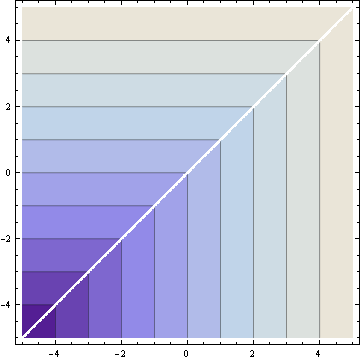
\includegraphics[width=2in]{./resources/hardmax.png}
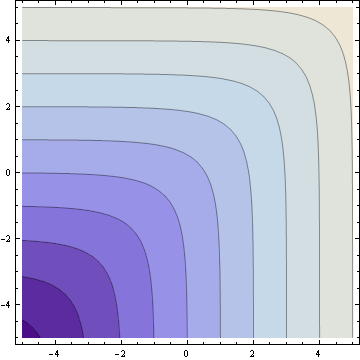
\includegraphics[width=2in]{./resources/softmax.png}
\end{center}
\end{figure}
\end{frame}

\begin{frame}
\frametitle{Multinomial Logit: Identification}
What is actually identified here?
\begin{itemize}
\item Helpful to look at the ratio of two choice probabilities
\begin{eqnarray*}
\log \frac{s_{ij}(\theta)}{s_{ik}(\theta)} = \mathbf{x_{ij}} \beta_j - \mathbf{x_{ik}} \beta_k \rightarrow  \mathbf{x_i}\cdot(\beta_j - \beta_k)
\end{eqnarray*}
\item We only identify the \alert{difference in indirect utilities} not the levels.
\item This is a feature and not a bug. Why?
\end{itemize}
\end{frame}

\begin{frame}
\frametitle{Multinomial Logit: Identification}
As another idea suppose we add a constant $C$ to each $\beta_j$.
\begin{eqnarray*}
s_{ij} = \frac{\exp[\mathbf{x_i} (\beta_j+C) ]}{\sum_k \exp[\mathbf{x_i} (\beta_k+C) ]} =  \frac{\exp[\mathbf{x_i} C] \exp[\mathbf{x_i} \beta_j ]}{\exp[\mathbf{x_i} C] \sum_k \exp[\mathbf{x_i} \beta_k ]} 
\end{eqnarray*}
\begin{itemize}
\item This has no effect.  That means we need to fix a normalization $C$. The most convenient is generally that $C = - \beta_K$. \
\item We normalize one of the choices to provide a utility of zero.
\item We actually already made another normalization. Does anyone know what?
\end{itemize}
\end{frame}


\begin{frame}
\frametitle{Multinomial Logit: Identification}
The most sensible normalization in demand settings is to allow for an \alert{outside option} which produces no utility in expectation.
\begin{eqnarray*}
s_{ij} = \frac{\exp[\mathbf{x_i}\beta_j ]}{1+\sum_k \exp[\mathbf{x_i} \beta_k ]} 
\end{eqnarray*}
\begin{itemize}
\item Hopefully the choice of outside option is well defined: not buying a yogurt, buying some other used car, etc.
\item Now this resembles the binomial logit model more closely.
\end{itemize}
\end{frame}


\begin{frame}{Back to Scale of Utility}
\begin{itemize}
\item Consider $U_{ij}^{*} = V_{ij} + \varepsilon_{ij}^{*}$ with $Var(\varepsilon^{*}) = \sigma^2 \pi^2/6$.
\item Without changing behavior we can divide by $\sigma$ so that $U_{ij} = V_{ij}/\sigma + \varepsilon_{ij}$ and $Var(\varepsilon^{*}/\sigma)=Var(\varepsilon) = \pi^2/6$
\begin{eqnarray*}
s_{ij} = \frac{e^{V_{ij}/\sigma}}{\sum_k e^{V_{ik}/\sigma}} \approx \frac{e^{\beta^{*}/\sigma \cdot x_{ij}}}{\sum_k e^{\beta^{*}/\sigma \cdot x_{ik}}}
\end{eqnarray*}
\item Every coefficient $\beta$ is rescaled by $\sigma$. This implies that only the ratio $\beta^{*}/\sigma$ is identified. 
\item Coefficients are relative to variance of unobserved factors. More unobserved variance $\longrightarrow$ smaller $\beta$.
\item Ratio $\beta_1/\beta_2$ is invariant to the scale parameter $\sigma$.
\end{itemize}
\end{frame}

\begin{frame}{Taste Variation}
\begin{itemize}
\item Logit allows for taste variation across individuals if two conditions are met: \alert{individual level data} and \alert{interact observed characteristics} only.
\item We often want to allow for something like $U_{ij} = x_{j} \beta_i - \alpha_i p_j + \varepsilon_{ij}$. 
\item We might want $\beta_i = \theta / y_i$ where $y_i$ is the income for individual $i$ or $\beta_i = \theta y_i$, etc.
\item Can also have $z_{ij}$ such as the distance between $i$ and hospital $j$.
\item Cannot have unobserved heterogeneity or heteroskedasticity in $\varepsilon_{ij}$.
\end{itemize}
\end{frame}

\begin{frame}{Taste Variation}
\begin{eqnarray*}
\frac{s_{ij}}{s_{ik}} = \frac{e^{V_{ij}}}{\sum_{k'} e^{V_{ik'}}} / \frac{e^{V_{ik}}}{\sum_{k'} e^{V_{ik'}}} = \frac{e^{V_{ij}}}{e^{V_{ik}}} = \exp[V_{ij} - V_{ik}].
\end{eqnarray*}
\begin{itemize}
\item The ratio of choice probabilities for $j$ and $k$ depends only on $j$ and $k$ and not on any alternative $l$, this is known as \alert{independence of irrelevant alternatives}.
\item For some (Luce (1959)) IIA was an attractive property for axiomatizing choice.
\item In fact the logit was derived in the search for a statistical model that satsified various axioms.
\end{itemize}
\end{frame}

\begin{frame}{IIA Property}
\begin{itemize}
\item The well known counterexample: You can choose to go to work on a car $c$ or blue bus $bb$. $P_{c} = P_{bb} = \frac{1}{2}$ so that $\frac{P_c}{P_{bb}} = 1$.
\item Now we introduce a red bus $rb$ that is identical to $bb$. Then $\frac{P_{rb}}{P_{bb}} = 1$ and $P_{c} = P_{bb}= P_{rb} = \frac{1}{3}$ as the logit model predicts.
\item In reality we don't expect painting a bus red would change the number of individuals who drive a car so we would anticipate $P_{c} = \frac{1}{2}$ and $P_{bb} = P_{rb} = \frac{1}{4}$.
\item We may not encounter too many cases where $\rho_{\varepsilon_{ik},\varepsilon_{ij}} \approx 1$, but we have many cases where this $\rho_{\varepsilon_{ik},\varepsilon_{ij}} \neq 0$
\item What we need is the ratio of probabilities to change when we introduce a third option!
\end{itemize}
\end{frame}

\begin{frame}{IIA Property}
\begin{itemize}
\item IIA implies that we can obtain consistent estimates for $\beta$ on any subset of alternatives.
\item This means instead of using all $J$ alternatives in the choice set, we could estimate on some subset $S \subset J$.
\item This used to be a way to reduce the computational burden of estimation (not clear this is an issue in 2016).
\item Sometimes we have \alert{choice based samples} where we oversample people who choose a particular alternative. Manski and Lerman (1977) show we can get consistent estimates for all but the ASC. This requires knowledge of the difference between the true rate $A_j$ and the choice-based sample rate $S_j$.
\item Hausman proposes a specification test of the logit model: estimate on the full dataset to get $\hat{\beta}$, construct a smaller subsample $S^k \subset J$ and $\hat{\beta^k}$ for one or more subsets $k$. If $|\hat{\beta}^k - \hat{\beta}|$ is small enough.
\end{itemize}
\end{frame}

\begin{frame}{IIA Property}
\begin{eqnarray*}
\frac{\partial s_{ij}}{\partial z_{ij}} = s_{ij}(1- s_{ij}) \frac{\partial V_{ij}}{\partial z_{ij}}
\end{eqnarray*}
And Elasticity:
\begin{eqnarray*}
\frac{ \partial \log s_{ij}}{ \partial \log z_{ij}} = s_{ij}(1- s_{ij}) \frac{\partial V_{ij}}{\partial z_{ij}} \frac{z_{ij}}{s_{ij}} = (1- s_{ij}) z_{ij} \frac{\partial V_{ij}}{\partial z_{ij}}
\end{eqnarray*}
With cross effects:
\begin{eqnarray*}
\frac{\partial s_{ij}}{\partial z_{ik}} = -s_{ij} s_{ik} \frac{\partial V_{ik}}{\partial z_{ik}}
\end{eqnarray*}
And Elasticity:
\begin{eqnarray*}
\frac{ \partial \log s_{ij}}{ \partial \log z_{ik}} = -s_{ik} z_{ik} \frac{\partial V_{ik}}{\partial z_{ik}}
\end{eqnarray*}
For the linear $V_{ij}$ case we have that $\frac{\partial V_{ij}}{\partial z_{ij}}=  \beta_z$.
\end{frame}

\begin{frame}{Proportional Substitution}
Cross elasticity doesn't really depend on $j$.
\begin{eqnarray*}
\frac{ \partial \log s_{ij}}{ \partial \log z_{ik}} = -s_{ik} z_{ik} \underbrace{\frac{\partial V_{ik}}{\partial z_{ik}}}_{\beta_z}.
\end{eqnarray*}
\begin{itemize}
\item This leads to the idea of proportional substitution. As option $k$ gets better it proportionally reduces the shares of the all other choices.
\item Likewise removing an option $k$ means that $\tilde{s}_{ij} = \frac{s_{ij}}{1-s_{ik}}$ for all other $j$.
\item This might be a desirable property but probably not.
\end{itemize}
\end{frame}





\begin{frame}
\frametitle{Multinomial Logit: Estimation with Individual Data}
Estimation is straightforward via Maximum Likelihood (MLE):
\begin{eqnarray*}
L(\mathbf{y} | \mathbf{x}, \theta) &=& \prod_{i=1}^N  \underbrace{\frac{n_i!}{\prod_{j=1}^J y_{ij}!}}_{C(\mathbf{y})} \prod_{j=1}^J  s_{ij}(x_{ij},\theta)^{y_{ij}} \\
ll(\mathbf{y} | \mathbf{x}, \theta) &=& \sum_{i=1}^N \log(C(\mathbf{y}))   + \sum_{i=1}^N \sum_{j=1}^J y_{ij} \log( s_{ij}(x_{ij},\theta)) \\
l(\mathbf{y} | \mathbf{x}, \theta) &\approx& \sum_{i=1}^N \sum_{j=1}^J y_{ij} \log( s_{ij}(x_{ij},\theta))
\end{eqnarray*}
\begin{itemize}
\item We can ignore the combinatorial term (with the factorials) since it does not affect the location of the maximum (it is additive and doesn't depend on $\theta$).
\end{itemize}
\end{frame}

\begin{frame}
\frametitle{Multinomial Logit: Inclusive Value}
To be more specific:
\begin{itemize}
\item Let's look a little more closely at what's going on:
\begin{eqnarray*}
\sum_{i=1}^N \sum_{j=1}^J  y_{ij} \left[ x_{ij} \beta - \underbrace{\log \left(\sum_{k=1}^K x_{ik} \beta  \right)}_{IV_i(\mathbf{x_i},\theta)} \right]
\end{eqnarray*}
\item We call the term on the right the \alert{logit inclusive value}. It does not depend on $k$ but might vary across choice situations/individuals $i$.
\item The point of the inclusive value is to guarantee that $\sum_{k=1} s_{ik}(\mathbf{x_i},\theta) = 1$.
\item If we somehow observed $IV_i(\theta)$ we could just do linear regression (in fact we could do this separately for each $K$).
\end{itemize}
\end{frame}


\begin{frame}
\frametitle{Multinomial Logit: Estimation with Aggregate Data}
Estimation is just like before
\begin{itemize}
\item  Suppose that all consumers had the same $x_{ij} = x_{j}$ (Choices depended only on products not on income, education, etc.)
\item We can construct $y_{j}^* = \sum_{i=1}^N y_{ij}$.
\begin{eqnarray*}
l(\mathbf{y} | \mathbf{x}, \theta) &\approx& \sum_{j=1}^J  y_{j}^{*} \log( s_{j}(\mathbf{x},\theta))
\end{eqnarray*}
\item When each consumer $i$ faces the same choice environment, we can aggregate data into \alert{sufficient statistics}.
\end{itemize}
\end{frame}


\begin{frame}
\frametitle{Multinomial Logit: Estimation with Aggregate Data}
\alert{Aggregation} is probably the most important property of the  logit:
\begin{itemize}
\item Instead of individual data, or a single group we might have multiple groups: if prices only change once per week, we can aggregate all of the week's sales into one ``observation''.
\item Likewise if we only observe that an individual is within one of five income buckets -- there is no loss from aggregating our data into these five buckets.
\item All of this depends on the precise form of $ s_{j}(\mathbf{x_i},\theta)$. When it doesn't change across observations: we can aggregate.
\item It functions as if we have a representative consumer up to $\varepsilon_{i}$.
\item We can use this idea to go from individual level to market demand: $q_j(\mathbf{x_i}) = N_i s_{ij}(\theta)$.
\end{itemize}
\end{frame}

\begin{frame}
\frametitle{Multinomial Logit: Elasticity}
An important output from a demand system are elasticities
\begin{itemize}
\item An important element in $\mathbf{x_i}$ are prices $[p_{1},\ldots,p_J]$
\item Helpful to write $u_{ij} = x_j \beta -\alpha p_j$ (assumes aggregation!).
\begin{eqnarray*}
\frac{\partial q_j}{\partial p_k} =-N \cdot \alpha \left(I[j = k] s_j -\sum_{k=1}^K s_j s_k \right)
\end{eqnarray*}
\item This implies that $ \eta_{jj} = \frac{\partial q_j}{\partial p_j} \frac{p_j}{q_j}  = -\alpha p_j (1-s_j)$.
\item The price elasticity is increasing in own price! (Why is this a bad idea?)
\item  $ \eta_{jk} = \frac{\partial q_j}{\partial p_k} \frac{p_k}{q_j}  = -\alpha p_k s_k$.
\item The cross price elasticity doesn't depend on which product $j$ you are talking about!
\end{itemize}
\end{frame}

\begin{frame}
\frametitle{Multinomial Logit: IIA}
The multinomial logit is frequently criticized for producing unrealistic substitution patterns
\begin{itemize}
\item Suppose we got rid of a product $k$ then $s_j^{(1)} = s_j^{(0)} \frac{1}{1- s_k}$.
\item Substitution is just proportional to your pre-existing shares $s_j$
\item No concept of ``closeness'' of competition!
\end{itemize}
\end{frame}

\begin{frame}
\frametitle{Can we do better?}
Multinomial Probit?
\begin{itemize}
\item The probit has $\varepsilon_i \sim N(0,\Sigma)$.
\item If $\Sigma$ is unrestricted, then this can produce relatively flexible substitution patterns.
\item Flexible is relative: still have normal tails, only pairwise correlations, etc.
\item It might be that $\rho_{12}$ is large if $1,2$ are similar products.
\item Much more flexible than Logit
\end{itemize}
Downside
\begin{itemize}
\item $\Sigma$ has potentially $J^2$ parameters (that is a lot)!
\item Maybe $J * (J-1)/2$ under symmetry. (still a lot).
\item Each time we want to compute $s_j(\theta)$ we have to simulate an integral of dimension $J$.
\item I wouldn't do this for $J \geq 5$.
\end{itemize}
\end{frame}

\begin{frame}
\frametitle{Relaxing IIA}
Let's make $\varepsilon_{ij}$ more flexible than IID. Hopefully still have our integrals work out.
\begin{eqnarray*}
u_{ij} =   x_{ij} \beta  + \varepsilon_{ij}
\end{eqnarray*}
\begin{itemize}
\item One approach is to allow for a block structure on $\varepsilon_{ij}$ (and consequently on the elasticities).
\item We assign products into groups $g$ and add a group specific error term
\begin{eqnarray*}
u_{ij} =   x_{ij} \beta  + \eta_{g} + \varepsilon_{ij}
\end{eqnarray*}
\item The trick putting a distribution on $\eta_g + \varepsilon_{ij}$ so that the integrals still work out.
\item Do not try this at home: it turns out the required distribution is known as \alert{GEV} and the resulting model is known as the \alert{nested logit}.
\end{itemize}
\end{frame}

\begin{frame}{Nested Logit}
A traditional (and simple) relaxation of the IIA property is the Nested Logit. This model is often presented as two sequential decisions.
\begin{itemize}
\item First consumers choose a category (following an IIA logit).
\item Within a category consumers make a second decision (following the IIA logit).
\item This leads to a situation where while choices within the same nest follow the IIA property (do not depend on attributes of other alternatives) choices among different nests do not!
\end{itemize}
\end{frame}

\begin{frame}{Alternative Interpretation}
\begin{figure}[htbp]
\begin{center}
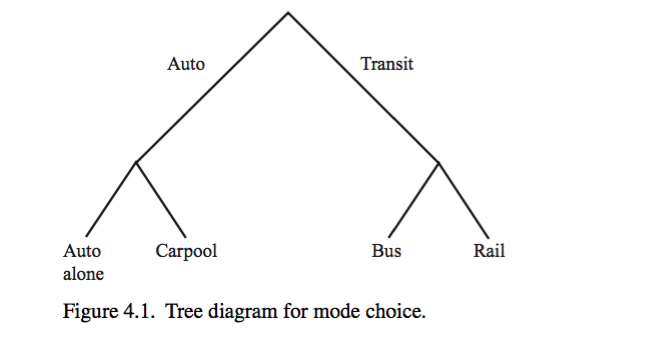
\includegraphics[width=5in]{resources/nesting.png}
\end{center}
\end{figure}
\end{frame}

\begin{frame}{Nested Logit}
Utility looks basically the same as before:
\begin{eqnarray*}
U_{ij} = V_{ij} + \underbrace{\eta_{ig} + \widetilde{\varepsilon_{ij}}}_{\varepsilon_{ij}(\lambda_g)}
\end{eqnarray*}
\begin{itemize}
\item We add a new term that depends on the group $g$ but not the product $j$ and think about it as varying unobservably over individuals $i$ just like $\varepsilon_{ij}$.
\item Now $\varepsilon_i \sim F(\varepsilon)$ where $F(\varepsilon) = \exp[-\sum_{g=G}^G \left(\sum_{j \in J_g} \exp[-\varepsilon_{ij}/\lambda_g]\right)^{\lambda_g}$. This is no longer Type I EV but GEV.
\item The key is the addition of the $\lambda_g$ parameters which govern (roughly) the within group correlation.
\item This distribution is a bit cooked up to get a closed form result, but for $\lambda_g \in [0,1]$ for all $g$ it is consistent with random utility maximization.
\end{itemize}
\end{frame}

\begin{frame}{Nested Logit}
The nested logit choice probabilities are:
\begin{eqnarray*}
P_{ij} = \frac{ e^{V_{ij}/\lambda_g} \left(\sum_{k \in J_g} e^{V_{ik}/\lambda_g} \right)^{\lambda_g -1}}{\sum_{h=1}^G \left(\sum_{k \in J_h} e^{V_{ik}/\lambda_h} \right)^{\lambda_h}}
\end{eqnarray*}
Within the same group $g$ we have IIA and proportional substitution 
\begin{eqnarray*}
\frac{P_{ij}}{P_{ik}} = \frac{ e^{V_{ij}/\lambda_g}}{ e^{V_{ik}/\lambda_g}}
\end{eqnarray*}

But for different groups we do not:
\begin{eqnarray*}
P_{ij} = \frac{ e^{V_{ij}/\lambda_g} \left(\sum_{k \in J_g} e^{V_{ik}/\lambda_g} \right)^{\lambda_g -1}}{ e^{V_{ik}/\lambda_h} \left(\sum_{k \in J_h} e^{V_{ik}/\lambda_h} \right)^{\lambda_h -1}}
\end{eqnarray*}
\end{frame}


\begin{frame}{Nested Logit}
We can take the probabilities and re-write them slightly with the substitution that 
$\lambda_g \cdot \underbrace{\log \left(\sum_{k \in J_g} e^{V_{ik}} \right)}_{IV_{ig}}$.
\begin{eqnarray*}
P_{ij} &=& \frac{ e^{V_{ij}/\lambda_g}}{ \left(\sum_{k \in J_g} e^{V_{ik}/\lambda_g} \right)}
\cdot
\frac{ \left(\sum_{k \in J_g} e^{V_{ik}/\lambda_g} \right)^{\lambda_g}}{\sum_{h=1}^G \left(\sum_{k \in J_h} e^{V_{ik}/\lambda_h} \right)^{\lambda_h}} \\
&=& \underbrace{\frac{ e^{V_{ij}/\lambda_g}}{ \left(\sum_{k \in J_g} e^{V_{ik}/\lambda_g} \right)}}_{P_{i j | g}}
\cdot
\underbrace{\frac{e^{\lambda_g IV_{ig}}}{\sum_{h=1}^{G} e^{\lambda_h IV_{ih}} }}_{P_{ig}}
\end{eqnarray*}
This is the decomposition into two logits that leads to the ``sequential logit'' story.
\end{frame}

\begin{frame}{Nested Logit : Notes}
\begin{itemize}
\item $\lambda_g=1$ is the simple logit case (IIA)
\item $\lambda_g \rightarrow 0$ implies that all consumers stay within the nest.
\item $\lambda < 0$ or $\lambda > 1$ can happen and usually means something is wrong. These models are not generally consistent with RUM. (If you report one in your paper I will reject it).
\item $\lambda$ is often interpreted as a correlation parameter and this is almost true but not exactly!
\item There are other extensions: overlapping nests, or three level nested logit. 
\item In general the hard part is understanding what the appropriate nesting structure is ex ante. Maybe for some problems this is obvious but for many not.
\end{itemize}
\end{frame}

%\begin{frame}{Nested Logit : Interpretation}
%\begin{itemize}
%\item It is convenient to think about the ``sequential choice'' version of the nested logit.
%\item In practice it is more accurate to think about the structure it imposes on the correlation of $\varepsilon_i$. 
%\item We specify a blocked structure (one block for each nest) and estimate a within vs. across nest correlation parameter.
%\end{itemize}
%\end{frame}


\begin{frame}
\frametitle{Nested Logit}
In practice we end up with the following:
\begin{eqnarray*}
s_{ij} = s_{ij|g}(\theta) s_{ig}(\theta)
\end{eqnarray*}
\begin{itemize}
\item Because the nested logit can be written as the within group share $s_{ij|g}$ and the share of the group $s_{ig}$ we often explain this model as \alert{sequential choice}
\item First you pick a category, then you pick a product within a category.
\item This is a sometimes helpful (sometimes unhelpful) way to think about this.
\item We can also think about this as putting a block structure on the covariance matrix of $\varepsilon_i$
\item You need to assign products to categories \alert{before you estimate} and you can't make mistakes!
\end{itemize}
\end{frame}

\begin{frame}
\frametitle{Nested Logit}
How does it actually look?
\begin{eqnarray*}
 IV_{ig}(\theta) &=& \log \left(\sum_{k \in G} \exp [x_k \beta/(1-\lambda_g)] \right) = E_{\varepsilon}[\max_{j \in G} u_{ij}]\\
 s_{ij|g}(\theta) &=& \frac{\exp [x_j \beta/(1-\lambda_g)]}{\sum_{k \in G} \exp [x_k \beta/(1-\lambda_g)]} \\
 s_{ig}(\theta) &=& \frac{\exp [IV_{ig}]^{1-\lambda_g}}{\sum_{h} \exp [IV_{ih}]^{1-\lambda_h}} 
\end{eqnarray*}
%\begin{itemize}
%\item When $\lambda_g \rightarrow 0$ we get the IIA logit model (no correlation within nests)
%\item When $\lambda_g \rightarrow 1$ we get no across nest substitution.
%\item When $\lambda_g > 1$ we get something not necessarily consistent with utility maximization!
%\end{itemize}
\end{frame}

\begin{frame}
\frametitle{Nested Logit}
How does it actually look?
\begin{eqnarray*}
\log \left(\frac{s_{ij|g}(\theta)}{s_{ik|g}(\theta)} \right) = (x_j -x_k)\cdot \frac{\beta}{1-\lambda_g}
 \end{eqnarray*}
 \begin{itemize}
\item We are back to having the IIA property but now within the group $G$.
\item We also have IIA across groups $g,h$
\item $\lambda_g$ and $\alpha$ govern the elasticities, which also have a block structure. % expand this later
\item Sometimes people refer to this as the \alert{product of two logits}
\item In the old days people used to estimate by fitting sequential IIA logit models -- this is consistent but inefficient -- you shouldn't do this today!
\item Estimation happens via MLE. This can be tricky because the model is non-convex. It helps to substitute $\tilde{\beta} = \beta/(1-\lambda_g)$
 \end{itemize}
\end{frame}

\begin{frame}
\frametitle{Parametric Identification}

Look at derivatives:
\begin{eqnarray*}
\frac{\partial\, s_{j|g}}{\partial X_j} &=& \beta_1 s_{j|g}(1-s_{j|g}) \\
 \frac{\partial\, s_{g}}{\partial X} &=& (1-\lambda) \beta_1 s_{g}(1-s_{g}) \\
  \frac{\partial\, s_{g}}{\partial J} &=& \frac{1-\lambda}{J} s_{g}(1-s_{g})
\end{eqnarray*}
\begin{itemize}
\item We get $\beta$ by changing $x_j$ within group
\item We get nesting parameter $\lambda$ by varying $X$
\item We don't have any parameters left to explain changing number of products $J$.
\end{itemize}

\end{frame}



\begin{frame}
\frametitle{Nested Logit}
There are more potential generalizations though they are less frequently used:
 \begin{itemize}
\item You can have multiple levels of nesting: first I select a size car (compact, mid-sized, full-sized) then I select a manufacturer, finally a car.
\item You can have potentially overlapping nests: Yogurt brands are one nest, Yogurt flavors are a second nest. This way strawberry competes with strawberry and/or Dannon substitutes for Dannon.
 \end{itemize}
\end{frame}


\begin{frame}
\frametitle{Mixed Logit}
We relax the IIA property by mixing over various logits:
\begin{eqnarray*}
u_{ijt} &=& x_j \beta + \mu_{ij} + \varepsilon_{ij} \\
s_{ij} &=& \int \frac{\exp[x_{j} \beta + \mu_{ij} ]}{1+\sum_k \exp[x_{k} \beta + \mu_{ik} ]} f(\mu_i | \theta)
\end{eqnarray*}
 \begin{itemize}
 \item Each individual draws a vector $\mu_i$ of $\mu_{ij}$ (separately from $\varepsilon$).
 \item Conditional on $\mu_i$ each person follows an IIA logit model.
 \item However we integrate (or mix) over many such individuals giving us a \alert{mixed logit} or \alert{heirarchical model} (if you are a statistician)
 \item In practice these are not that different from linear \alert{random effects models} you have learned about previously.
 \item It helps to think about fixing $\mu_i$ first and then integrating out over $\varepsilon_i$
 \end{itemize}
\end{frame}

\begin{frame}{Mixed/ Random Coefficients Logit}
As an alternative, we could have specified an error components structure on $\varepsilon_i$.
\begin{eqnarray*}
U_{ij} = \beta x_{ij} + \underbrace{\nu_i z_{ij} + \varepsilon_{ij}}_{\tilde{\varepsilon}_{ij}}
\end{eqnarray*}
\begin{itemize}
\item The key is that $\nu_i$ is unobserved and mean zero. But that $x_{ij},z_{ij}$ are observed per usual and $\varepsilon_{ij}$ is IID Type I EV.
\item This allows for a heteroskedastic structure on $\varepsilon_{i}$, but only one which we can project down onto the space of $z$.
\end{itemize}
An alternative is to allow for individuals to have random variation in $\beta_i$:
\begin{eqnarray*}
U_{ij} = \beta_i x_{ij} +  \varepsilon_{ij}
\end{eqnarray*}
Which is the random coefficients formulation (these are the same model).
\end{frame}

%
%\begin{frame}{Mixed/ Random Coefficients Logit}
%For each individual $i$, the resulting choice probability follows a logit:
%\begin{eqnarray*}
%P_{ij} = \int \frac{ e^{V_{ij}(\beta_i)}}{\sum_k e^{V_{ik}(\beta_i)}} f(\beta_i | \theta) \partial \beta
%\end{eqnarray*}
%This structure is quite general:
%\begin{itemize}
%\item The choice probabilities are know a function of unknown parameters $\theta$.
%\item We can allow for there to be two types of $\beta_i$ in the population (high-type, low-type). \alert{latent class model}.
%\item We can allow $\beta_i$ to follow an independent normal distribution for each component of $x_{ij}$ such as $\beta_i = \overline{\beta} + \nu_i \sigma$.
%\item We can allow for correlated normal draws using the Cholesky root of the covariance matrix.
%\item Can allow for non-normal distributions too (lognormal, exponential). Why is normal so easy?
%\end{itemize}
%\end{frame}

\begin{frame}{Mixed/ Random Coefficients Logit}
\begin{itemize}
\item Kinds of heterogeneity
\begin{itemize}
\item We can allow for there to be two types of $\beta_i$ in the population (high-type, low-type). \alert{latent class model}.
\item We can allow $\beta_i$ to follow an independent normal distribution for each component of $x_{ij}$ such as $\beta_i = \overline{\beta} + \nu_i \sigma$.
\item We can allow for correlated normal draws using the Cholesky root of the covariance matrix.
\item Can allow for non-normal distributions too (lognormal, exponential). Why is normal so easy?
\end{itemize}
\item The structure is extremely flexible but at a cost.
\item We generally must perform the integration numerically.
\item High-dimensional numerical integration is difficult. In fact, integration in dimension 8 or higher makes me very nervous.
\item We need to be parsimonious in how many variables have unobservable heterogeneity.
\item Again observed heterogeneity does not make life difficult so the more of that the better!
\end{itemize}
\end{frame}

\begin{frame}
\frametitle{Mixed Logit}
How does it work?
 \begin{itemize}
\item Well we are mixing over individuals who conditional on $\beta_i$ or $\mu_i$ follow logit substitution patterns, however they may differ wildly in their $s_{ij}$ and hence their substitution patterns.
\item For example if we are buying cameras: I may care a lot about price, you may care a lot about megapixels, and someone else may care mostly about zoom.
\item The basic idea is that we need to explain the heteroskedasticity of $Cov(\varepsilon_i, \varepsilon_j)$ what random coefficients do is let us use a basis from our $X$'s.
\item If our $X$'s are able to span the space effectively, then an RC logit model can approximate any arbitrary RUM (McFadden and Train 2002). 
\item Of course if you have 1000 products and two random coefficients, you are asking for a lot.
 \end{itemize}
\end{frame}


%\begin{frame}{Mixed/ Random Coefficients Logit}
%How do we approximate:
%\begin{eqnarray*}
%P_{ij} = \int \frac{ e^{V_{ij}(\beta_i)}}{\sum_k e^{V_{ik}(\beta_i)}} f(\beta_i | \theta) \partial \beta
%\end{eqnarray*}
%
%\begin{itemize}
%\item Monte Carlo Integration
%\begin{itemize}
%\item Draw $\beta_i$ from the candidate distribution. $[\beta_i^{(1)}, \beta_i^{(2)}, \ldots\beta_i^{(s)}] | \theta$.
%\item For each $\beta_i$ calculate $P_{ij}(\beta_i)$.
%\item $\frac{1}{S} \sum_{s=1}^S P_{ij} = \widehat{P_{j}^{s}}$
%\end{itemize}
%\end{itemize}
%The way we usually get correlated normal variables (or any normal variables) is to transform independent normals appropriately.
%\end{frame}

\begin{frame}{Mixed/ Random Coefficients Logit}
Suppose there is only one random coefficient, and the others are fixed:
\begin{itemize}
\item $f(\beta_i \theta) \sim N(\overline{\beta},\sigma)$.
\item We can re-write this as the integral over a transformed standard normal density
\begin{eqnarray*}
P_{ij}(\theta) = \int \frac{ e^{V_{ij}(\nu_i,\theta)}}{\sum_k e^{V_{ik}(\nu_i,\theta)}} f(\nu_i) \partial \nu
\end{eqnarray*}
\item Monte Carlo Integration: Independent Normal Case
\begin{itemize}
\item Draw $\nu_i$ from the standard normal distribution.
\item Now we can rewrite $\beta_i = \overline{\beta} + \nu_i \sigma$
\item For each $\beta_i$ calculate $P_{ij}(\beta_i)$.
\item $\frac{1}{S} \sum_{s=1}^S P_{ij} = \widehat{P_{j}^{s}}$
\end{itemize}
\item Gaussian Quadrature
\begin{itemize}
\item Or we can draw a non-random set of points $\nu_i$ and corresponding weights $w_i$ and approximate the integral to a high level of polynomial accuracy.
\end{itemize}
\end{itemize}
\end{frame}

\begin{frame}{Quadrature in higher dimensions}
\begin{itemize}
\item Quadrature is great in low dimensions -- but scales badly in high dimensions.
\item If we need $N_a$ points to accurately approximate the integral in $d=1$ then we need $N_a^d$ points in dimension $d$ (using the tensor product of quadrature rules).
\item There is some research on quadrature rules that nest and also how to carefully eliminate points so that the number doesn't grow so quickly.
\item Try \url{sparse-grids.de}
\end{itemize}
\end{frame}

\begin{frame}{Estimation}
How do we actually estimate these models?
\begin{itemize}
\item In practice we should be able to do MLE.
\begin{eqnarray*}
\max_{\theta} \sum_{i=1}^N y_{ij} \log P_{ij}(\theta)
\end{eqnarray*}
\item When we are doing IIA logit, this problem is globally convex and is easy to estimate using Newton's Method.
\item When doing nested logit or random coefficients logit, it generally is non-convex which can make life difficult.
\item The tough part is generally working out what $\frac{\partial \log P_{ij}}{\partial \theta}$ is, especially when we need to simulate to obtain $P_{ij}$.
\item It turns out that MSLE actually has consistent problems for fixed $S$. Why?
\item Alternative? MSM/MoM type estimators (next time).
\end{itemize}
\end{frame}




%\begin{frame}
%\frametitle{Mixed Logit}
% \begin{itemize}
%\item Now the choice of $\mu_{ij}$ is crucial.  
%\item A popular choice is \alert{random coefficients logit}: $\beta_i = \overline{\beta} +  \Sigma \nu_i * \mathbf{x_j}$ where $\nu_i$ is a vector of standard normal draws and $\Sigma$ are covariance parameters so that $\beta_i \sim N(\overline{\beta},\Sigma)$.
%\item We have to estimate $(\overline{\beta},\Sigma)$.
%\item People are often lazy and let $\Sigma$ be a diagonal matrix to reduce the \# of parameters.
% \end{itemize}
%\end{frame}


\begin{frame}
\frametitle{Mixed Logit: Estimation}
 \begin{itemize}
\item Just like before, we do MLE
\item One wrinkle--how do we compute the integral?
 \end{itemize}
\begin{eqnarray*}
s_{ij} &=& \int \frac{\exp[x_{j} \beta_i  ]}{1+\sum_k \exp[x_{k} \beta_i  ]} f(\beta_i | \theta) \\
 &=& \sum_{s=1}^{ns} w_s \frac{\exp[x_{j} (\overline{\beta} + \Sigma \nu_{is})  ]}{1+\sum_k \exp[x_{k} (\overline{\beta} + \Sigma \nu_{is})  ]} 
\end{eqnarray*}
 \begin{itemize}
\item Option 1: Monte Carlo integration.  Draw $NS=1000$ or so samples of $\nu_i$ from the standard normal and set $w_i = \frac{1}{NS}$.
\item Option 2: Quadrature. Choose $\nu_i$ and $w_i$ according to a Gaussian quadrature rule. Like \texttt{quad} in MATLAB.
\item Personally I get nervous about integrals in dimension greater than 5. People routinely have 20 or more though.
 \end{itemize}
\end{frame}

\begin{frame}
\frametitle{Mixed Logit: Hints}
 How bad is the simulation error?
 \begin{itemize}
\item Depends how small your shares are. 
\item Since you care about $\log s_{jt}$ when shares are small, tiny errors can be enormous.
\item Often it is pretty bad.
\item I recommend sticking with quadrature at a high level of precision.
\item \texttt{sparse-grids.de} provide efficient high dimensional quadrature rules.
 \end{itemize}
\end{frame}

\subsection{A Semiparametric Estimator}

\begin{frame}
\frametitle{Even More Flexibility (Fox, Kim, Ryan, Bajari)}
Suppose we wanted to nonparametrically estimate $f(\beta_i | \theta)$ instead of assuming that it is normal or log-normal.
\begin{eqnarray*}
s_{ij} &=& \int \frac{\exp[x_{j} \beta_i  ]}{1+\sum_k \exp[x_{k} \beta_i  ]} f(\beta_i | \theta)
\end{eqnarray*}
\begin{itemize}
\item Choose a distribution $g(\beta_i)$ that is more spread out that $f(\beta_i | \theta)$
\item Draw several $\beta_{s}$ from that distribution (maybe 500-1000).
\item Compute $\hat{s}_{ij}(\beta_s)$ for each draw of $\beta_s$ and each $j$.
\item Holding $\hat{s}_{ij}(\beta_s)$ fixed, look for $w_s$ that solve
\begin{eqnarray*}
\min_w \left(s_j -  \sum_{s=1}^{ns} w_s \hat{s}_{ij}(\beta_s) \right)^2 \quad \mbox{ s.t. } \sum_{s=1}^{ns} w_s = 1, \quad w_s \geq 0 \quad \forall s
\end{eqnarray*}
\end{itemize}
\end{frame}

\begin{frame}
\frametitle{Even More Flexibility (Fox, Kim, Ryan, Bajari)}
% Hey this is lasso
\begin{itemize}
\item Like other semi-/non- parametric estimators, when it works it is both general and very easy.
\item We are solving a least squares problem with constraints: positive coefficients, coefficients sum to 1.
\item It tends to produce \alert{sparse models} with only a small number of $\beta_s$ getting positive weights.
\item This is way easier than solving a random coefficients logit model with all but the simplest distributions.
\item There is a bias-variance tradeoff in choosing $g(\beta_i)$.
\item Incorporating parameters that are not random coefficients loses some of the simplicity.
\item I have no idea how to do this with large numbers of fixed effects.
\end{itemize}
\end{frame}



\section{Convexity and Computation}
\frame{\frametitle{Convexity}
\begin{block}{An optimization problem is convex if}
\begin{eqnarray*}
\min_{x} f(\mathbf{x}) &s.t.& h(\mathbf{x}) \leq 0 \quad A \mathbf{x} = 0
\end{eqnarray*}
\vskip -2ex
\begin{itemize}
\item $f(\mathbf{x}),h(\mathbf{x)}$ are convex (PSD second derivative matrix)
\item Equality Constraint is affine
\end{itemize}
\end{block}
\begin{exampleblock}{Some helpful identities about convexity}
\begin{itemize}
\item Compositions  and sums of convex functions are convex.
\item Norms $||$ are convex, $\max$ is convex, $\log$ is convex
\item  $ \log(\sum_{i=1}^n \exp(x_i))$ is convex.
\item Fixed Points can introduce non-convexities.
\item Globally convex problems have a unique optimum
\end{itemize}
\end{exampleblock}
}

\frame{\frametitle{Properties of Convex Optimization}
\begin{itemize}
\item If a program is globally convex then it has a unique minimizer that will be found by convex optimizers.
\item If a program is not globally convex, but is convex over a region of the parameter space, then most convex optimization routines find any local minima in the convex hull 
\item Convex optimization routines are unlikely to find local minima (including the global minimum) if they do not begin in the same convex hull as the optimum (starting values matter!).
\item Most good commercial routines are clever about dealing with multiple starting values and handling problems that are well approximated by convex functions.
\item Good Routines use information about sparseness of Hessian -- this generally determines speed.
\end{itemize}
}

\subsection{Nested Logit Example}


%\subsection{Logit and Nested Logit}
%\frame{\frametitle{Logit Model}
%Easy to see that FIML estimator is convex:
%\begin{eqnarray*}
%\min_{\theta} \sum_j q_j \ln \left(\frac{\exp[x_j \beta ]}{1+\sum_j \exp[x_j \beta]} \right)\\
%\min_{\theta} \sum_j q_j \left( x_j \beta  - \ln \left(1+\sum_j \exp[x_j \beta ]\right) \right)\\
%\end{eqnarray*}
%}

\frame{\frametitle{Nested Logit Model}
\begin{exampleblock}{FIML Nested Logit Model is Non-Convex}
\begin{eqnarray*}
\min_{\theta} \sum_j q_j \ln P_j(\theta) \quad \mbox{s.t.} \quad  P_j(\theta) = \frac{e^{x_j \beta/ \lambda}( \sum_{k \in g_l} e^{x_j \beta/ \lambda})^{\lambda-1}}{\sum_{\forall l'} ( \sum_{k \in g_l'} e^{x_j \beta/ \lambda})^{\lambda} }
\end{eqnarray*}
This is a pain to show but the problem is with the cross term $\frac{\partial^2 P_j}{\partial \beta \partial \lambda}$ because $\exp[x_j \beta / \lambda]$ is not convex.
\end{exampleblock}
\begin{exampleblock}{A Simple Substitution Saves the Day:  let $\gamma = \beta / \lambda$}
\begin{eqnarray*}
\min_{\theta} \sum_j q_j \ln P_j(\theta) \quad \mbox{s.t.} \quad  
P_j(\theta) = \frac{e^{x_j \gamma}( \sum_{k \in g_l} e^{x_j \gamma})^{\lambda-1}}{\sum_{\forall l'} ( \sum_{k \in g_l'} e^{x_j \gamma})^{\lambda} }
\end{eqnarray*}
This is much better behaved and easier to optimize.
\end{exampleblock}
}

\frame{\frametitle{Nested Logit Model}
\begin{center}
\rowcolors[]{1}{RoyalBlue!10}{RoyalBlue!20} 
\begin{tabular}{lrrr}
&\bf{Original}\footnote{KNITRO-AMPL} & \bf{Substitution}\footnote{KNITRO-AMPL} & \bf{No Derivatives}\footnote{fminunc-MATLAB} \\
Parameters &49& 49&49\\
Nonlinear $\lambda$ &5 &5 &5\\
Likelihood & 2.279448 &2.279448  & 2.27972\\
Iterations &197 &146 & 352\\
Time & 59.0 s & 10.7 s & 192s  \\
\end{tabular}
\end{center}
Discuss Nelder-Meade
}

\frame{\frametitle{Computing Derivatives}
A key aspect of any optimization problem is going to be computing the derivatives (first and second) of the model.  There are some different approaches
\begin{itemize}
\item Numerical: Often inaccurate and error prone (why?)
\item Pencil and Paper: this tends to be mistake prone -- but often actually the fastest
\item Automatic (AMPL): Software brute forces through a chain rule calculation at every step (limited language).
\item Symbolic (Maple/Mathematica): software ``knows'' derivatives of certain objects and can do its own simplification.  (limited language).
\end{itemize}
}


\end{document}